\documentclass{beamer}
\usetheme{metropolis}
\usepackage{graphicx}
\usepackage{subfig}
\usepackage{tcolorbox}
\title{Computer Logic and Digital Circuit Design (PHYS306/COSC330): Unit 2.2}
\author{Jordan Hanson}
\institute{Whittier College Department of Physics and Astronomy}

\begin{document}
\maketitle

\section{Summary}

\begin{frame}{Unit 2.2 Summary - Theoretical Logic Gates, and Operations}
\textbf{Reading: DF Chapter 3-4 (Moodle)}
\begin{enumerate}
\item Logic Gates
\begin{itemize}
\item Circuit diagram
\item Truth table
\item Timing diagram
\item Boolean logic
\end{itemize}
\item \alert{Boolean algebra I}
\item IC Circuits, \textbf{data sheets}
\item \alert{Boolean algebra II}
\end{enumerate}
\textbf{Homework: Chapter 3, ex. 1-22 (two weeks)}
\end{frame}

\section{Fixed-Function Logic: IC Gates}

\begin{frame}{Fixed-Function Logic: IC Gates}
IC Gates are an interesting but fading topic.
\begin{enumerate}
\item Some basic realities
\item Notions of power and time
\item \alert{Fun with part numbers and data-sheets}
\begin{itemize}
\item \textit{This may not seem as important, but it is}
\end{itemize}
\end{enumerate}
\end{frame}

\begin{frame}{Fixed-Function Logic: IC Gates}
\textit{Switching time - $t_s$}, \textit{Power dissipation - $P_d = V^2/R$} \\ \vspace{0.5cm}
\begin{columns}[T]
\begin{column}{0.5\textwidth}
CMOS \\ \hrulefill
\begin{itemize}
\item Complementary Metal-Oxide Semiconductor
\item MOSFETs
\item Lower \textit{power dissipation}
\item 3.3V and 5V type (voltage that represents HIGH)
\end{itemize}
\end{column}
\begin{column}{0.5\textwidth}
TTL \\ \hrulefill
\begin{itemize}
\item Transistor-Transistor Logic
\item BJTs
\item Faster \textit{switching speeds}
\item 5V type (voltage that represents HIGH)
\end{itemize}
\end{column}
\end{columns}
\hrulefill \\
Chapter 3 examines 54/74 series IC gates.
\end{frame}

\begin{frame}{Fixed-Function Logic: IC Gates}
Chapter 3 examines 54/74 series IC gates. \\ \vspace{0.5cm}
\framebox[1.1\width]{\url{www.digikey.com}} \\ \vspace{0.5cm}
Sample part number: \textbf{74}\textit{A}\alert{LV}\textbf{\alert{C}}20
\begin{itemize}
\item \textbf{74} Mil-spec or military specification.  54 is commerical specification
\item \textit{A} ``Advanced''
\item \alert{LV} low-voltage (3.3 V type), could also be HV or high-voltage (5.0 V type)
\item \textbf{\alert{C}} CMOS, could also be CT for TTL compatibility
\item 20: specific gates inside.  In this case we have two NAND gates with 4-inputs each
\end{itemize}
\end{frame}

\begin{frame}{Fixed-Function Logic: IC Gates}
\begin{table}
\begin{tabular}{c c}
\textbf{End code} & \textbf{IC contents} \\ \hline
00 & Quad 2-input NAND \\
02 & Quad 2-input NOR \\
04 & Hex inverter \\
08 & Quad 2-input AND \\
10 & Triple 3-input NAND \\
11 & Triple 3-input AND \\
20 & Dual 4-input NAND \\
21 & Dual 2-input AND \\
27 & Triple 3-input NOR \\
30 & Single 8-input NAND \\
32 & Quad 2-input OR \\
86 & Quad 2-input XOR
\end{tabular}
\end{table}
\end{frame}

\begin{frame}{Fixed-Function Logic: IC Gates}
\small
Chapter 3 examines 54/74 series IC gates. \\ \vspace{0.5cm}
\framebox[1.1\width]{\url{www.digikey.com}} Get the data sheets. \\ \vspace{0.5cm}
Sample part number: \textbf{74}\textit{A}\alert{LV}\textbf{\alert{C}}20
\begin{enumerate}
\item Look up power dissipation.  Can't find it?  Then find $I_{CCL}$ and/or $I_{CCH}$.
\item Look up propagation delay time $t_d$.  Usually it is in nanoseconds.
\item Look up voltage type (\textit{does it match}?)
\item $P_D = V_{cc} \left(\frac{I_{CCL} + I_{CCH}}{2}\right)$
\item Compute the speed-power product (SPP) (product of the delay time and $P_D$)
\item Repeat (6) for a variety of part numbers, and plot (SPP) versus $t_d$ and $P_D$.
\end{enumerate}
\end{frame}

\begin{frame}{Fixed-Function Logic: IC Gates}
\small
Chapter 3 examines 54/74 series IC gates. \\ \vspace{0.5cm}
\framebox[1.1\width]{\url{www.digikey.com}} Get the data sheets. \\ \vspace{0.5cm}
Sample part number: \textbf{74}\textit{A}\alert{LV}\textbf{\alert{C}}20
\begin{enumerate}
\item Look up power dissipation.  Can't find it?  Then find $I_{CCL}$ and/or $I_{CCH}$.
\item Look up propagation delay time $t_d$.  Usually it is in nanoseconds.
\item Look up voltage type (\textit{does it match}?)
\item $P_D = V_{cc} \left(\frac{I_{CCL} + I_{CCH}}{2}\right)$
\item Compute the speed-power product (SPP) (product of the delay time and $P_D$)
\item Repeat (6) for a variety of part numbers, and plot (SPP) versus $t_d$ and $P_D$.
\end{enumerate}
\end{frame}

\begin{frame}{Fixed-Function Logic: IC Gates}
\small
Chapter 3 examines 54/74 series IC gates. \\ \vspace{0.5cm}
\framebox[1.1\width]{\url{www.digikey.com}} Get the data sheets. \\ \vspace{0.5cm}
Sample part number: \textbf{74}\textit{A}\alert{LV}\textbf{\alert{C}}20
\begin{enumerate}
\item Compute fan-out:
\begin{equation}
UL = \frac{I_{OH}}{I_{IH}} = \frac{I_{OL}}{I_{IL}}
\end{equation}
This is the ratio of input and output currents in the low and high states.  Represents the maximum number of down-stream gates a given gate can handle.
\item CMOS systems are ``high-impedance'' (high-resistance) so the fan-out should be high.  Think about this in terms of Ohm's law ($V=iR$).
\item Compute fan-out for a variety of part numbers
\end{enumerate}
\end{frame}

\begin{frame}{Fixed-Function Logic: IC Gates}
\alert{\textbf{The key to this lesson is that data sheets and part numbers matter.  It's not just gibberish.}} \\ \vspace{1cm}
Imagine buying 54-series parts, because that's what they last guy did, building a unit, and deploying it in...Antarctica.  What's the temperature in Antarctica?  Yeah...you needed to buy 74-series. \\ \vspace{1cm}
Also, an important feature of any IC/digital component data sheet is the \textbf{pin-out.}
\end{frame}

\begin{frame}{Fixed-Function Logic: IC Gates}
\begin{figure}
\centering
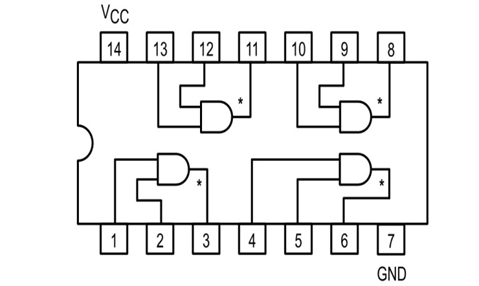
\includegraphics[width=0.8\textwidth]{figures/Quad2NAND.png}
\caption{\label{fig:Q2N.png} Example of IC \textit{pinout}, which displays \textbf{which pins mean what.}}
\end{figure}
\end{frame}

\begin{frame}{Fixed-Function Logic: IC Gates}
Vocabulary recap:
\begin{enumerate}
\item Pinout
\item Ohm's Law
\item SPP
\item $t_d$
\item $P_d$
\item $I_{IH}$, $I_{OH}$
\item $I_{IL}$, $I_{OL}$
\item $V_{CC}$, $I_{CCL}$, $I_{CCH}$ (which current is higher?)
\item CMOS, TTL, MOSFET
\end{enumerate}
\end{frame}

\section{Conclusion}

\begin{frame}{Unit 2.2 Summary - Theoretical Logic Gates, and Operations}
\textbf{Reading: DF Chapter 3-4 (Moodle)}
\begin{enumerate}
\item Logic Gates
\begin{itemize}
\item Circuit diagram
\item Truth table
\item Timing diagram
\item Boolean logic
\end{itemize}
\item \alert{Boolean algebra I}
\item IC Circuits, \textbf{data sheets}
\item \alert{Boolean algebra II}
\end{enumerate}
\textbf{Homework: Chapter 3, ex. 1-22 (two weeks)}
\end{frame}

\end{document}
